	\section{Nombre: Piso congelado}\label{obs.pisoC}
	\subsection{Descripción}
	Porción de suelo. Cuando el jugador camina sobre este obstáculo, la fricción entre el jugador y el obstáculo disminuye provocando que la velocidad de desplazamiento del jugador se incremente y que cuando el jugador se detenga no lo haga de golpe sino resbale una distancia determinada antes de detenerse.
	\subsection{Esquema}
	Ver figura \ref{fig:pisoC}.
	\begin{figure}
		\centering
		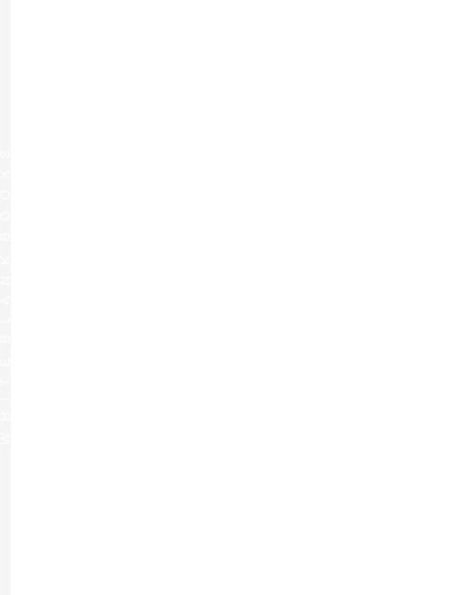
\includegraphics[height=0.2 \textheight]{Imagenes/pisoC}
		\caption{Piso congelado.}
		\label{fig:pisoC}
	\end{figure}